\documentclass[12pt]{ctexart}
\usepackage{ctex}
%\usepackage{txfonts} 这个里面不能用,原因不明
\usepackage [nottoc]{tocbibind}
\usepackage{graphicx}
\usepackage{amsmath}
\usepackage{float}
\usepackage{geometry}
\geometry{a4paper,centering,scale=0.8}

%\usepackage[format=hang,font=small,textfont=it]{caption}
\newtheorem{thm}{定理}
\title{勾股定理} 
\author{\kaishu \zihao{3} 苏有朋}
\date{\today}

\newenvironment{myquote}{\begin{quote}\kaishu\zihao{4}}{\end{quote}}

%\usepackage{cite}
\bibliographystyle{plain}
\begin{document}
	\maketitle
	\begin{abstract}
		这是一篇关于勾股定理的小短文
		grap
		实时编译结果查看
		撒娇的哈师大
	\end{abstract}
	\newpage
	
	\tableofcontents
	\newpage
	
	\section{勾股定理在古代}
	西方称勾股定理为毕达哥拉斯定理,将勾股定理的发现归功于公元前6世纪的毕达哥拉斯学派\cite{Kline}。该学派得到了一个法则,可以求出可排成直角三角形三边的三元数组。毕达哥拉斯学派没有书面著作,该定理的严格表述和证明则见于欧几里德\footnote{欧几里得,约公元前330--275年}《几何原本》的命题47:“直角三角形斜边上的正方形等于两直角边上的两个正方形之和。”证明是用面积做的。\\
	
	我国《周辞算经》载商高(约公元前12世纪)答周公问:
	\begin{myquote}
		勾广三,股修四,径隅五。
	\end{myquote}%不能有\\

	又载陈子(约公元前7--6世纪)答荣方问:\cite{quanjing}
	\begin{quote}
		\emph{若求邪至日者,以日下为勾,日高为股,勾股各自乘,并而开方除之,得邪至日。}
	\end{quote}
	都较古希腊更早。
	\newpage
	
	\section{勾股定理的近代形式}
	\eqref{eq:gougu}······的整数称为\emph{勾股数}\\%eqref公式的引用
	
	\begin{thm}[勾股定理]
		直角三角形斜边的平方等于两腰的平方和。可以用符号语言描述为
	\end{thm}

	\begin{eqnarray}\label{eq:gougu}
		a^2+b^2=c^2\\
		\angle ABC = \pi/2(90^{\circ})
	\end{eqnarray}
	\begin{figure}[ht]
		\centering 
		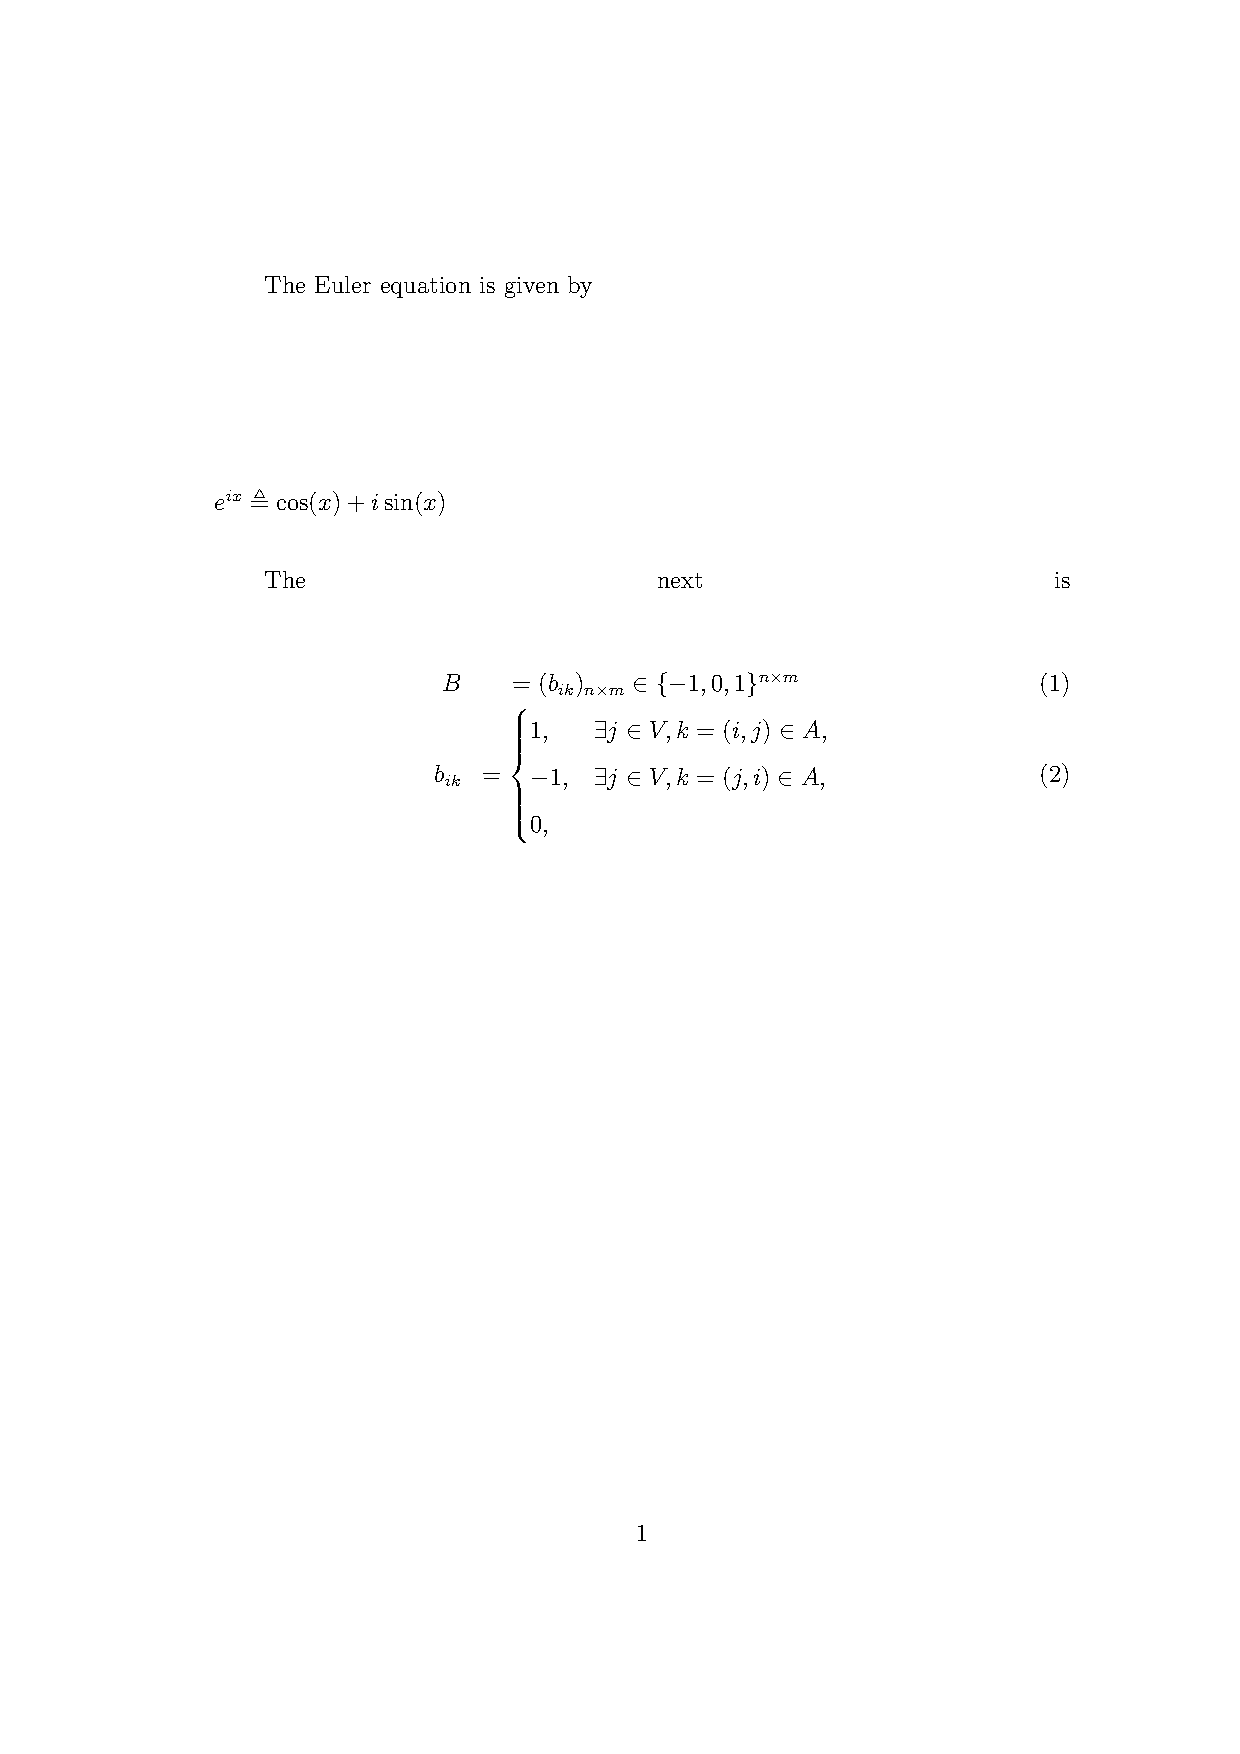
\includegraphics[width=12cm]{aaa.pdf}
		\caption{宋赵爽在《周律算经》注中作的弦图(仿制),该图给出了勾股定理的一个极具对称美的证明。}
		\label{fig:xiantu}
	\end{figure}

	\begin{table}[h]
		\centering
	\begin{tabular}{|c|c|c|}
		\hline
		直角边a&直角边b&斜边c\\
		\hline
		3&4&5\\
		5&12&13\\
		\hline
	\end{tabular}
	\end{table}

	\qquad $a^2+b^2=c^2$
	\newpage
	\nocite{shiye}
	\bibliography{math}
\end{document}